\subsubsection{Subproceso 3.B: Confirmaci\'on y Registro Oficial}

El modelo BPMN del Subproceso 3.B distribuye el proceso actual en cinco carriles, los mismos actores de la secci\'on 3: el Estudiante Regular, la Oficina de Estad\'istica de la Facultad, la Direcci\'on de Registro Central y Estad\'istica (DIRCE), los Docentes de Asignatura y los organismos nacionales SUNEDU y MINEDU. La Oficina de Estad\'istica concentra la parte operativa del cierre: inscribe las autorizaciones de la primera semana, recaba la estad\'istica por secci\'on, comunica el cierre y env\'ia el archivo digital de consolidaci\'on, visa el Reporte y la Boleta y prepara los padrones de clase. La DIRCE registra la matr\'icula en el SIGA, resuelve las modificaciones extempor\'aneas, genera los documentos oficiales, env\'ia el padr\'on nacional a SUNEDU y MINEDU y entrega al final el registro actualizado a las Facultades. El estudiante solo interviene al inicio, con la entrega de la Pre-Ficha, y los docentes reciben el padr\'on de su asignatura y secci\'on.

Esta vista vertical reproduce la misma secuencia del diagrama de flujo, ahora con la responsabilidad de cada actor. Suma un matiz relevante: si el visado sale no conforme, el Reporte o la Boleta vuelven a observaci\'on y reproceso hasta obtener la conformidad, de modo que el proceso tiene un \'unico evento de fin, la matr\'icula oficializada.

\begin{figure}[H]
    \centering
    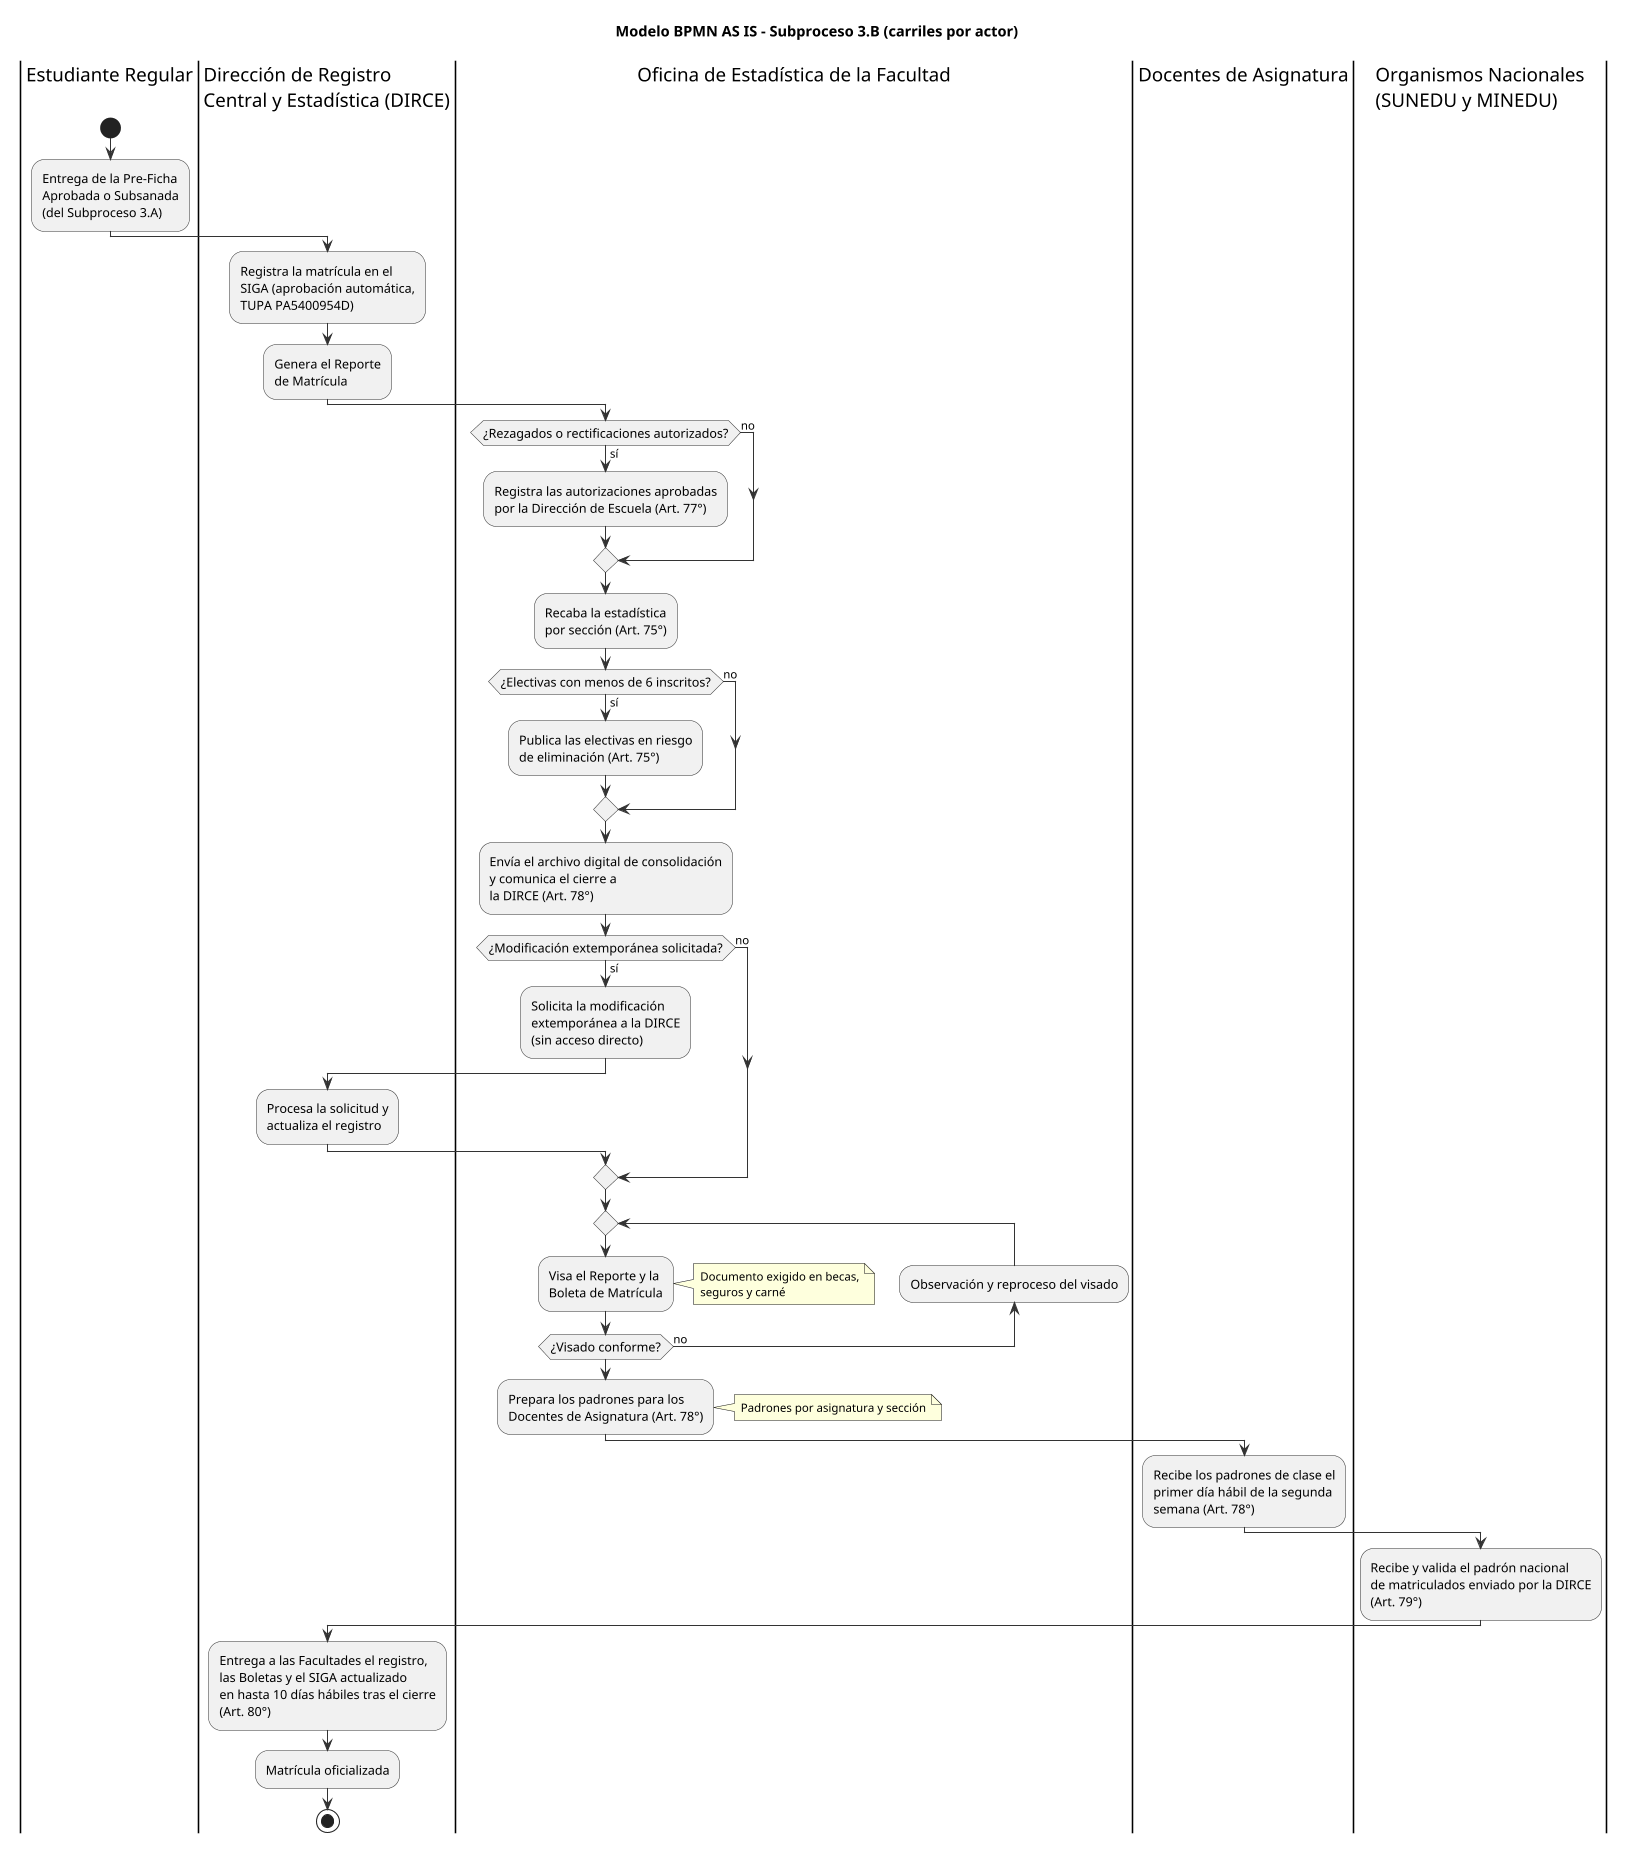
\includegraphics[width=0.9\textwidth]{asis_subproceso_3b_bpmn.png}
    \caption{Modelo BPMN vertical (AS IS) del Subproceso 3.B}
    \label{fig:asis_3b_bpmn}
\end{figure}
